% =============================================================
%  Detección de Residuos Urbanos — versión en español (2 col.)
%  Compilar: pdflatex main_es && bibtex main_es && pdflatex main_es ×2
% =============================================================
\documentclass[conference]{IEEEtran}

\usepackage[utf8]{inputenc}
\usepackage[T1]{fontenc}
\usepackage[spanish,es-tabla]{babel}
\usepackage{graphicx}
\usepackage{booktabs}
\usepackage{multirow}
\usepackage{amsmath}
\usepackage{xcolor}
\usepackage[colorlinks=true, citecolor=blue, urlcolor=blue, linkcolor=blue]{hyperref}
\usepackage{tikz}
\usetikzlibrary{positioning, arrows.meta}

\graphicspath{{../figuras_final/}{../figuras_eda/}{../figuras_p0/}{../figuras_p1/}}

\renewcommand{\IEEEkeywordsname}{Palabras clave}

\begin{document}

\title{¿Qué tan lejos viaja un detector de basura?\\
Detección cross-domain de residuos urbanos en imágenes de mano, dashcam y dron}

\author{
\IEEEauthorblockN{Jairzinho Santos}
\IEEEauthorblockA{Universidad Nacional de Ingenier\'ia, Lima, Per\'u\\
Visi\'on Computacional --- Maestr\'ia en Inteligencia Artificial, 2026-I}}

\maketitle

% =============================================================
\begin{abstract}
El monitoreo automatizado de basura suele evaluarse dentro de un solo dominio de
imagen, pero los despliegues reales mezclan reportes ciudadanos, cámaras
vehiculares y drones. Estudiamos cuánto se degradan los detectores de residuos
urbanos entre tres dominios públicos ---TACO (mano), RoLID-11K (dashcam) y
UAVVaste (dron)--- bajo un único protocolo auditado de evaluación. Nuestra
curación destapó siete defectos en los datasets publicados, en particular fuga a
nivel de video en los splits oficiales de RoLID-11K: el 58.2\,\% del test
comparte video de origen con el entrenamiento, y un modelo entrenado con ese
traslape obtiene +21\,\% de AP$_{50}$ sobre el mismo test. Comparamos Faster
R-CNN, un segmentador FCN e interpretabilidad basada en CAM contra una
referencia YOLOv11, y medimos una degradación cross-domain de 82\,\% en
mAP$_{50}$, dominada por la escala de los objetos (mediana de 22\,px en dashcam,
por debajo del ancla FPN más pequeña). Elevar la resolución a 1024\,px recupera
hasta 8.3 puntos de AP$_{50}$ y 5.8 de AP$_S$. Publicamos código, pesos y splits
auditados.
\end{abstract}

\begin{IEEEkeywords}
detección de basura, evaluación cross-domain, auditoría de datasets, objetos pequeños
\end{IEEEkeywords}

% =============================================================
\section{Introducción}
La basura no recolectada afecta la salud pública, el turismo y los presupuestos
municipales, y su monitoreo aún depende de inspección manual de cobertura
limitada. La visión computacional promete monitoreo continuo y de bajo costo, y
el trabajo reciente ha producido datasets públicos de detección de basura en
escenarios complementarios: fotografías de mano a nivel de calle
(TACO~\cite{taco}), dashcams frontales (RoLID-11K~\cite{rolid}), imágenes de
dron (UAVVaste~\cite{uavvaste}) y cámaras ojo de pez en camiones recolectores
(StreetView-Waste~\cite{streetview}). Cada benchmark, sin embargo, se evalúa
\emph{dentro de su dominio}; si un detector entrenado en un punto de vista sigue
siendo útil en otro ---la situación que enfrenta cualquier ciudad que despliegue
sensores mixtos--- no había sido medido.

Este trabajo pregunta: \emph{¿cuánto se degrada la detección de basura urbana
entre dominios de imagen, y qué importa más para cerrar la brecha: la
arquitectura, la resolución de entrada o la higiene de los datos de
entrenamiento?} Responderla exigió más que entrenar detectores. Auditar los tres
datasets destapó siete defectos (Sección~\ref{sec:data}), incluida la fuga a
nivel de video en los splits oficiales de RoLID-11K que infla los baselines
publicados, colisiones de nombres de archivo y marcos de anotación EXIF
inconsistentes en TACO y UAVVaste. Construimos por ello un pipeline de curación
auditado con splits congelados conscientes de grupos, y evaluamos todos los
modelos contra los mismos ground truths.

Nuestras contribuciones son:
(i) una auditoría documentada de tres datasets públicos de basura, con splits
corregidos y publicados;
(ii) la primera matriz de evaluación cross-domain entre imágenes de mano,
dashcam y dron;
(iii) la cuantificación de la inflación por fuga en el protocolo oficial de
RoLID-11K (+21\,\% de AP$_{50}$ por memorización de escena);
(iv) una comparación controlada de detectores clásicos afinados, segmentación e
interpretabilidad contra una referencia moderna en tiempo real, incluyendo una
ablación de resolución para objetos pequeños y un estudio de granularidad de
clases (6 contra 5 clases de material).

% =============================================================
\section{Trabajo relacionado}
\textbf{Datasets de basura.} TACO~\cite{taco} aporta 1{,}500 imágenes de mano
con 60 categorías y polígonos de segmentación. RoLID-11K~\cite{rolid} contribuye
11.5k cuadros de dashcam con una sola clase \emph{litter} y estadísticas
marcadas de objeto pequeño. UAVVaste~\cite{uavvaste} cubre vistas de dron a baja
altura. StreetView-Waste~\cite{streetview} apunta a cámaras ojo de pez de
camiones recolectores; sus enlaces de descarga no estuvieron disponibles durante
este trabajo. Detect-waste~\cite{detectwaste} armonizó varias de estas fuentes;
ZeroWaste~\cite{zerowaste} aborda la clasificación industrial, un dominio que
excluimos deliberadamente.

\textbf{Detección bajo restricciones.} TrashDet~\cite{trashdet} busca detectores
TinyML sobre TACO y alcanza 19.5 de mAP$_{50}$ en un subconjunto de cinco
clases: evidencia de que las cifras absolutas de este problema son
estructuralmente bajas, lo que motiva nuestro énfasis en cantidades
\emph{relativas} entre dominios. Los autores de RoLID evalúan detectores
modernos, con cabezas transformer (CO-DETR) superando a las variantes YOLO por
más de 20 puntos de AP$_{50}$, consistente con el régimen extremo de objetos
pequeños.

\textbf{Métodos.} Nos apoyamos en Faster R-CNN~\cite{fasterrcnn} y su RPN, la
segmentación totalmente convolucional~\cite{fcn}, la interpretabilidad por
activación de clase~\cite{cam,gradcam,guidedbp}, YOLOv11~\cite{yolo11} como
referencia en tiempo real, TIDE~\cite{tide} para descomponer el error y la
estratificación iterativa~\cite{sechidis} para particiones conscientes de
grupos.

% =============================================================
\section{Datasets, auditoría y curación}
\label{sec:data}

Ingerimos los tres datasets del alcance mediante un pipeline tipo medallón
(raw$\rightarrow$bronze$\rightarrow$silver$\rightarrow$gold) con manifiestos por
capa y linaje SHA-256; la Figura~\ref{fig:pipeline} resume el flujo completo,
de la ingesta verificada al contrato de evaluación.

\begin{figure*}[t]
\centering
\begin{tikzpicture}[
  caja/.style={draw=black!55, rounded corners=2pt, align=center,
               font=\scriptsize, inner sep=4pt, minimum height=9mm},
  fl/.style={-{Stealth[length=2mm]}, black!65, semithick},
  et/.style={font=\tiny, black!60},
  node distance=5mm and 5mm]
\node[caja, fill=black!4] (src) {Fuentes p\'ublicas\\Zenodo · Drive · GitHub};
\node[caja, fill=black!4, right=of src] (raw) {\textbf{raw}\\inmutable · MD5};
\node[caja, fill=black!4, right=of raw] (bronze) {\textbf{bronze}\\navegable};
\node[caja, fill=blue!6, right=of bronze] (silver) {\textbf{silver}\\auditor\'ia H1--H7 · C1--C5\\splits congelados por grupos};
\node[caja, fill=orange!10, right=of silver] (gold) {\textbf{gold}\\pools 1280 · dirs YOLO\\GT COCO · m\'ascaras · recortes};
\node[caja, fill=blue!6, below=8mm of bronze] (mac) {\textbf{carril Mac} (MPS)\\VGG E1--E4 · FCN D1--D2\\YOLO F1};
\node[caja, fill=blue!6, right=of mac] (colab) {\textbf{carril Colab} (A100)\\Faster R-CNN A/B/C\\YOLO F2--F4, G, H};
\node[caja, fill=green!7, right=of colab] (eval) {\textbf{contrato de evaluaci\'on}\\pycocotools vs.\ GT congelados\\descomposici\'on TIDE};
\node[caja, fill=green!7, right=of eval] (res) {\textbf{19 corridas DONE}\\matriz · fuga\\ablaci\'on · 6-vs-5};
\draw[fl] (src) -- node[et, above]{00} (raw);
\draw[fl] (raw) -- (bronze);
\draw[fl] (bronze) -- node[et, above]{01--02} (silver);
\draw[fl] (silver) -- node[et, above]{03} (gold);
\draw[fl] (gold.south) to[out=-90, in=90] node[et, right, pos=0.35]{04--05} (colab.north);
\draw[fl] (gold.south west) to[out=-120, in=45] (mac.north east);
\draw[fl] (mac) -- (colab);
\draw[fl] (colab) -- node[et, above]{06} (eval);
\draw[fl] (eval) -- (res);
\node[et, below=1mm of mac.south, xshift=18mm]
  {guardianes de presupuesto, NaN y cuarentena enrutan las corridas entre carriles};
\end{tikzpicture}
\caption{Pipeline de punta a punta. Los datos fluyen por una arquitectura medall\'on
con linaje SHA-256 (etiquetas de flecha: n\'umeros de notebook); el entrenamiento
corre en dos carriles gobernados por guardianes autom\'aticos; todos los modelos
se eval\'uan bajo un solo contrato m\'etrico.}
\label{fig:pipeline}
\end{figure*}
 La Tabla~\ref{tab:domains} resume los dominios y la Figura~\ref{fig:scale} muestra el eje que los separa: la escala del objeto.

\begin{table}[t]
\caption{Los tres dominios tras la curación. Lado mediano de objeto medido
sobre el pool de entrenamiento de 1280 px.}
\label{tab:domains}
\centering
\small
\begin{tabular}{lcccc}
\toprule
Dataset & Vista & Imágenes & Obj.\ med. & \% small \\
\midrule
TACO & mano & 1{,}500 & 171 px & 25 \\
RoLID-11K & dashcam & 11{,}564 & \textbf{22 px} & 84 \\
UAVVaste & dron & 772 & 72 px & 66 \\
\bottomrule
\end{tabular}
\end{table}

\begin{figure}[t]
\centering
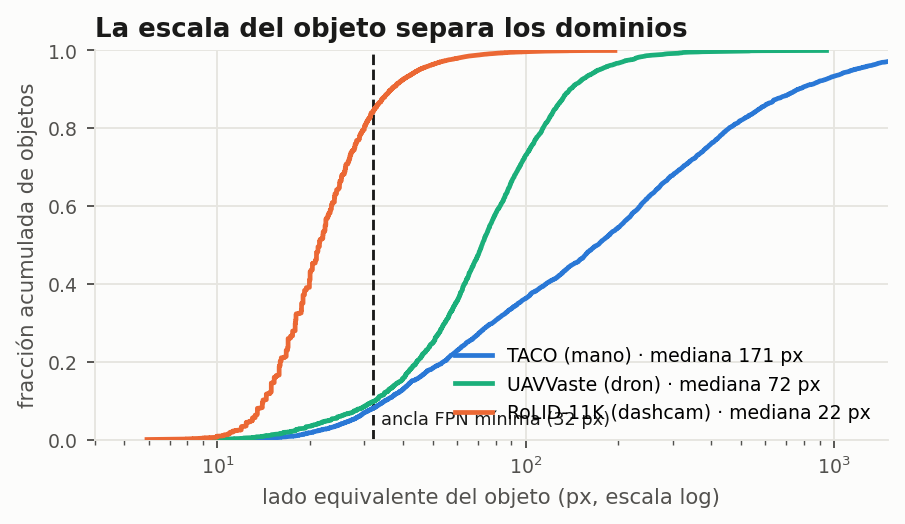
\includegraphics[width=\linewidth]{escala_objetos.png}
\caption{Distribución acumulada del lado del objeto por dominio. La
mediana de RoLID (22\,px) cae bajo el ancla FPN mínima de 32\,px: el
régimen que explica la matriz cross-domain y motiva la ablación de
resolución.}
\label{fig:scale}
\end{figure}


\textbf{Hallazgos de la auditoría.} Verificaciones sistemáticas (hashing
perceptual, verificación de marcos EXIF, cruce de splits) destaparon siete
defectos que corregimos o documentamos: (H1) los nombres de archivo de TACO
colisionan entre lotes (92\,\% de las imágenes comparte nombre con otro lote);
(H2) $\sim$37\,\% de las imágenes de TACO trae rotaciones EXIF pendientes, con
cajas anotadas sobre el marco \emph{rotado}; (H3) las carpetas de la
distribución de RoLID no codifican la hora de captura; (H4) \textbf{los splits
oficiales de RoLID fugan a nivel de video}: 22 de 84 videos de origen abarcan
varios splits y el 58.2\,\% de los cuadros de test comparte video con el
entrenamiento ---cuadros casi duplicados (87\,\% de redundancia visual por hash
perceptual) convierten esto en fuga de escena que infla los baselines
publicados; (H5) una imagen está duplicada entre val y test oficiales; (H6) el
split oficial de UAVVaste también contiene un par casi duplicado que cruza
train/test; (H7) los marcos de anotación son inconsistentes entre datasets
---TACO anota sobre el marco rotado por EXIF mientras que cinco fotos de mano de
UAVVaste anotan el marco crudo---, por lo que los píxeles se materializan por
imagen en el marco que coincide con las dimensiones declaradas, con los
metadatos EXIF removidos.

\textbf{Curación.} Silver aplica cinco correcciones (duplicado removido de val,
categoría fantasma eliminada, identidad por ruta completa, marcado de caja
degenerada y de duplicados MD5), define una taxonomía de dos niveles
---\emph{litter} (1 clase, todos los datasets) y clases de material de TACO en
dos variantes paralelas, \textbf{A: 6 clases} (con vidrio, marginal con 38
instancias proyectadas de test) y \textbf{B: 5 clases} (sin vidrio)--- y congela
cuatro esquemas de split con unidades conscientes de grupo: grupos visuales
pHash para TACO/UAVVaste y \emph{video de origen} para RoLID. Los splits de TACO
usan estratificación iterativa~\cite{sechidis}; cada clase cae a menos de 0.1
puntos del objetivo de 15\,\% de test. Para RoLID mantenemos \emph{ambos}
esquemas, el oficial (con fuga, por comparabilidad) y el por-video (0\,\% de
fuga), lo que habilita la cuantificación pareada de la inflación.

% =============================================================
\section{Métodos}
\label{sec:methods}

\textbf{P0 --- pipeline clásico afinado.}
(1)~\emph{Faster R-CNN} (ResNet-50-FPN, preentrenado en COCO) bajo dos
estrategias de transferencia ---backbone congelado contra descongelar
\texttt{layer4}--- con warmup lineal, recorte de gradiente y early stopping
sobre el AP$_{50}$ de validación.
(2)~\emph{FCN-ResNet18} para segmentación binaria basura/fondo sobre los
polígonos rasterizados de TACO (conv $1\times1$ + conv transpuesta $\times$32
con inicialización bilineal, entropía cruzada ponderada por clase).
(3)~\emph{Transfer learning con VGG-16} sobre recortes de 224 px basura/fondo
(dos estrategias $\times$ dos tasas de aprendizaje), sustrato de los paneles de
interpretabilidad CAM~\cite{cam}, Grad-CAM~\cite{gradcam} y Guided
Backpropagation~\cite{guidedbp}.
(4)~Un \emph{análisis de cobertura de anclas}: las anclas base de FPN
(32--512 px) contra las distribuciones medidas de tamaño de objeto, más mapas de
objectness del RPN del modelo dashcam entrenado ---una explicación mecanicista
de la brecha de objetos pequeños.

\textbf{P1 --- referencia moderna.} YOLOv11n~\cite{yolo11} entrenado por dominio
a 640 px (y 1024 px para la ablación de resolución), usado para llenar la matriz
cross-domain $3\times3$, el par oficial-contra-por-video de la fuga y la
comparativa de variantes 6-contra-5 clases.

\textbf{Contrato de evaluación.} Una sola fuente de verdad métrica: las
predicciones de todos los modelos se evalúan con herramientas COCO contra los
mismos ground truths congelados; el test se toca una vez por experimento con los
pesos de mejor validación; las predicciones guardadas alimentan la
descomposición de errores TIDE~\cite{tide}.

% =============================================================
\section{Configuración experimental}
Diecinueve corridas (11 de P0, 8 de P1) ejecutadas en dos carriles: Apple
M-series (MPS) para VGG/FCN/YOLO y CUDA (Colab A100) para Faster R-CNN y las
corridas YOLO pesadas ---el perfilado mostró iteraciones sanas de Faster R-CNN
de $\sim$95\,s en MPS (las entradas de tamaño variable fuerzan recompilación de
kernels por forma) contra $\sim$0.3\,s en CUDA; un guardián de presupuesto en
horas proyectó el costo total tras la primera época y desvió automáticamente las
corridas inviables. Presupuestos: topes generosos de épocas (50--150) con early
stopping (paciencia 8--30) y curvas de validación; semillas fijas; checkpoints
por época con reanudación. Las imágenes se materializan a lado máximo de 1280
(Lanczos, JPEG q95) en el marco de anotación (H7). La Figura~\ref{fig:curves} muestra las trayectorias de validación de las
ocho corridas YOLO: convergencia limpia, early stopping actuando y la
separación por dominio y resolución.

\begin{figure}[t]
\centering
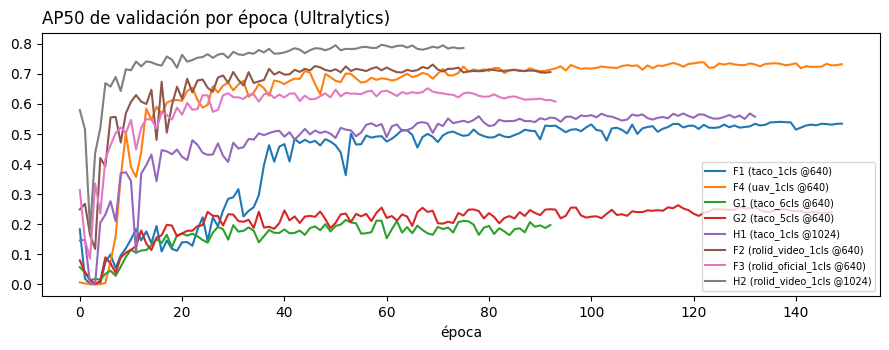
\includegraphics[width=\linewidth]{../figuras_p1/p1_curvas.png}
\caption{AP$_{50}$ de validación por época de las ocho corridas YOLOv11n.}
\label{fig:curves}
\end{figure}

Los exports multiclase
excluyen \emph{negativos envenenados} ---imágenes cuyos únicos objetos
pertenecen a clases excluidas--- en lugar de entrenarlos como fondo (1/38/60
imágenes para las variantes de 1/6/5 clases).

% =============================================================
\section{Resultados}
\label{sec:results}
Cada número de esta sección lo genera la notebook de evaluación consolidada a
partir de las predicciones de test guardadas contra los ground truths
congelados; ninguna métrica se transcribe a mano.

\subsection{Matriz cross-domain}
La Figura~\ref{fig:matrix} presenta el resultado central. Dentro de dominio, los
tres modelos YOLOv11n promedian 0.639 de AP$_{50}$; entre dominios la cifra se
desploma a 0.118: una \textbf{degradación de 82\,\%}. La matriz es fuertemente
asimétrica: el dominio dashcam es una isla (AP$_{50}\!\le\!0.064$ en ambas
direcciones), mientras que mano$\rightarrow$dron transfiere sorprendentemente
bien (0.527, reteniendo el 68\,\% del puntaje in-domain del dron). El patrón
señala a la \emph{escala del objeto} antes que a la apariencia: los objetos de
TACO y UAVVaste (medianas de 171 y 72\,px) caen dentro del rango de anclas de
FPN, mientras que la mediana de 22\,px de RoLID queda por debajo del ancla
mínima de 32\,px ---consistente con nuestro análisis de cobertura de anclas y
con que AP$_S$ colapsa más fuerte (AP$_S$ diagonal: 0.056 / 0.279 / 0.374).

\begin{figure}[t]
\centering
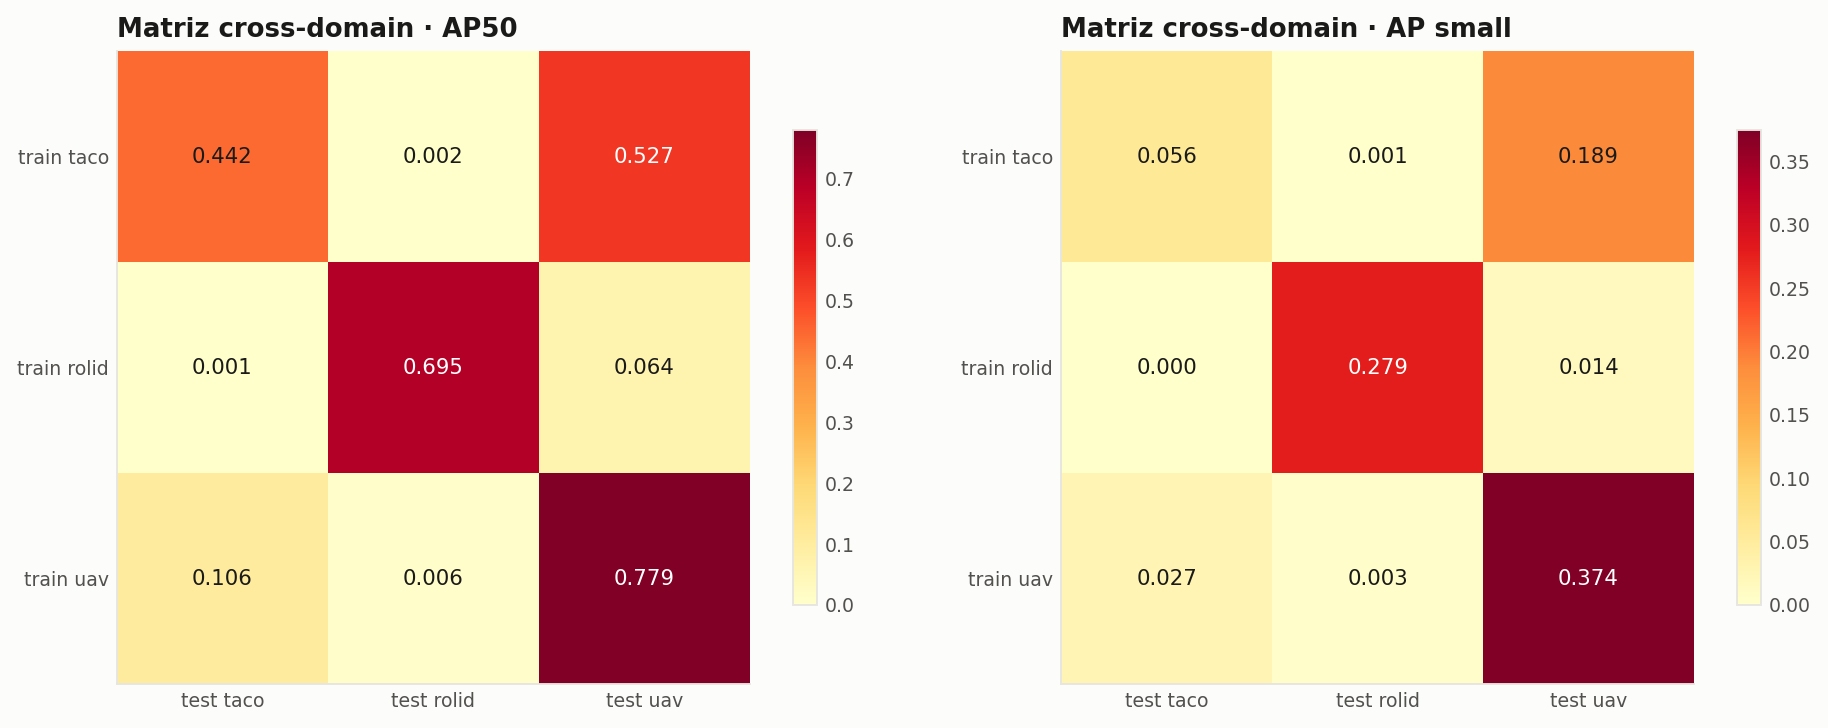
\includegraphics[width=\linewidth]{matriz_cross_domain_final.png}
\caption{Matriz cross-domain en test (YOLOv11n @640): AP$_{50}$
(izquierda) y AP$_S$ (derecha). Filas: dominio de entrenamiento;
columnas: dominio de test. Media in-domain 0.639 contra 0.118 cruzada.}
\label{fig:matrix}
\end{figure}

\subsection{Inflación por fuga en RoLID-11K}
La Tabla~\ref{tab:leak} aparea los protocolos oficial (58\,\% de fuga de video)
y por-video (0\,\%). Sobre el \emph{mismo} test limpio por-video, el modelo
entrenado con el split oficial ---que vio otros cuadros de esos mismos videos de
test--- obtiene 0.844 de AP$_{50}$ contra 0.695 del modelo entrenado limpio: una
\textbf{inflación relativa de +21\,\%} atribuible a memorización de escena y no
a generalización (el 87\,\% de los pares de cuadros intra-video son visualmente
redundantes por hash perceptual). Los baselines publicados sobre el protocolo
oficial deben leerse con este sesgo presente; el split consciente de grupos lo
elimina a costo cero.

\begin{table}[t]
\caption{Cuantificación de la fuga en RoLID-11K (AP$_{50}$ de test,
YOLOv11n @640).}
\label{tab:leak}
\centering
\small
\begin{tabular}{llc}
\toprule
Split de entrenamiento & Test & AP$_{50}$ \\
\midrule
oficial (58\,\% fuga) & oficial & 0.620 \\
por video (0\,\% fuga) & por video & 0.695 \\
oficial (58\,\% fuga) & por video & \textbf{0.844} \\
\bottomrule
\end{tabular}
\end{table}

\subsection{Familias bajo el mismo protocolo}
La Tabla~\ref{tab:families} compara Faster R-CNN (41.3\,M de parámetros) y
YOLOv11n (2.6\,M) sobre splits y ground truths idénticos. En tareas de una sola
clase el modelo 16$\times$ más pequeño queda a 1--4 puntos de AP$_{50}$ (0.695
contra 0.707 en dashcam; 0.442 contra 0.483 en mano), lo que respalda el
despliegue ligero; en clasificación de materiales la brecha se abre a 5--9
puntos. Descongelar \texttt{layer4} eleva a Faster R-CNN en +3.7 de AP$_{50}$
sobre el backbone congelado (0.483 contra 0.446). Nuestro YOLO de 5 clases
(0.192 de mAP$_{50}$) es consistente con el 19.5 de TrashDet en un subconjunto
comparable de TACO~\cite{trashdet}, confirmando que las cifras absolutas del
problema son estructuralmente bajas. Los modelos complementarios de P0 cierran
el cuadro: FCN-ResNet18 alcanza 0.577 de IoU de test en segmentación binaria de
basura, y el clasificador de recortes VGG-16 llega a 97.8\,\% de exactitud de
test, dando el sustrato para la evidencia CAM/Grad-CAM de que la red atiende al
objeto y no al contexto (Figura~\ref{fig:cam}).

\begin{figure}[t]
\centering
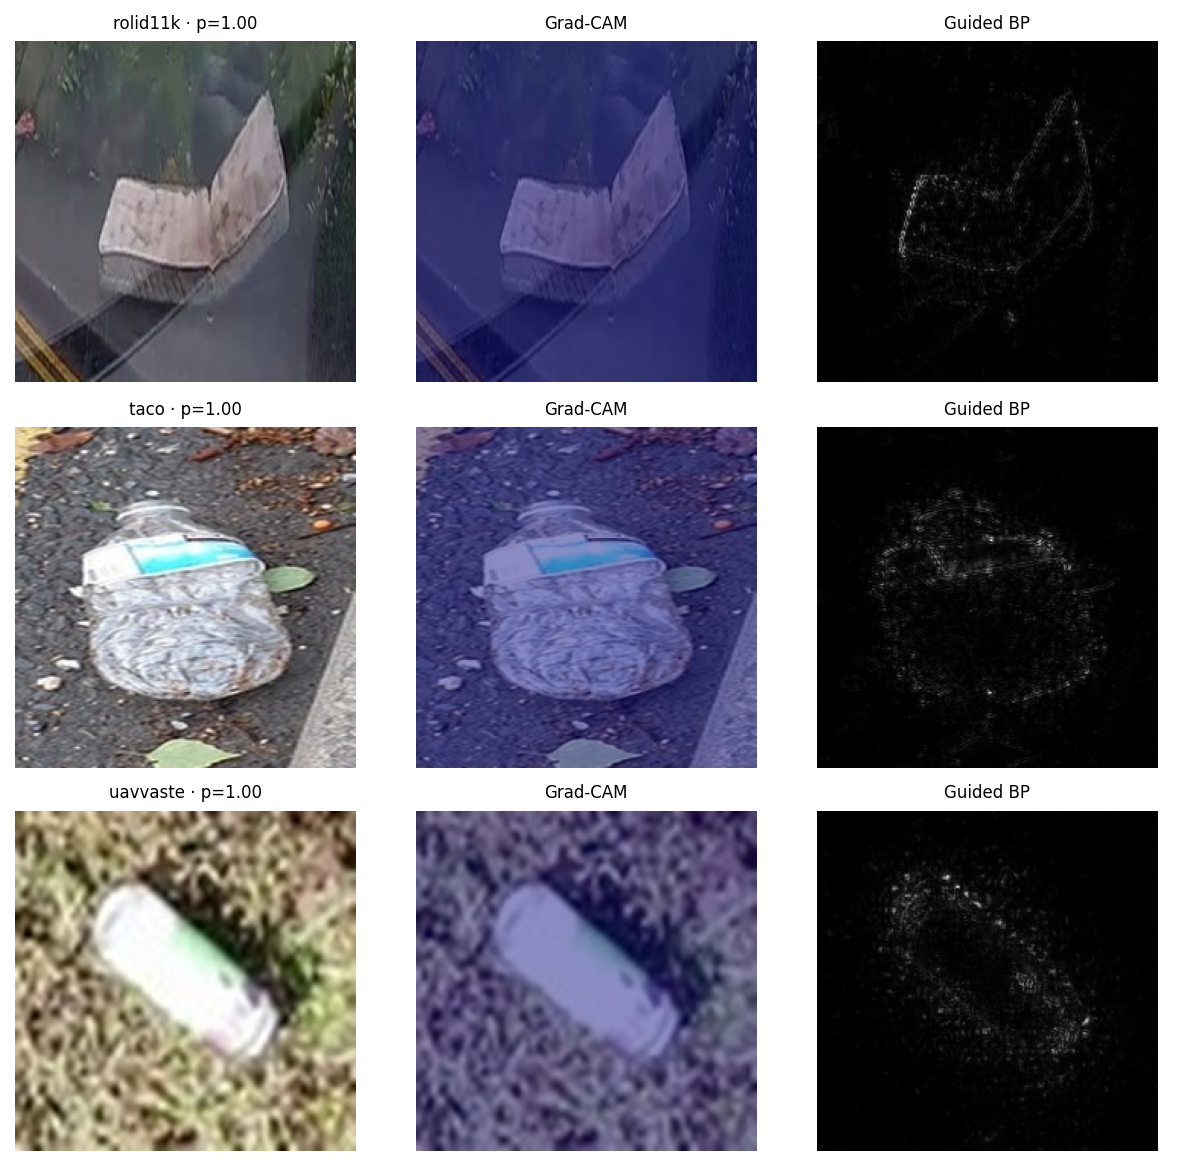
\includegraphics[width=\linewidth]{cam_panel_paper.png}
\caption{Interpretabilidad del clasificador de recortes: una fila por
dominio (dashcam, mano, dron) con Grad-CAM y Guided Backpropagation. La
activación se concentra en el objeto incluso en los recortes de 22\,px.}
\label{fig:cam}
\end{figure}

\begin{table}[t]
\caption{Familias de modelos sobre splits idénticos (métricas de test).
FRCNN = Faster R-CNN R50-FPN con \texttt{layer4} descongelada.}
\label{tab:families}
\centering
\small
\begin{tabular}{llccc}
\toprule
Datos & Modelo & AP$_{50}$ & AP & AP$_S$ \\
\midrule
\multirow{2}{*}{TACO 1 clase} & FRCNN & \textbf{0.483} & \textbf{0.323} & \textbf{0.073} \\
 & YOLOv11n & 0.442 & 0.318 & 0.056 \\
\midrule
\multirow{2}{*}{RoLID por video} & FRCNN & \textbf{0.707} & 0.277 & \textbf{0.281} \\
 & YOLOv11n & 0.695 & \textbf{0.279} & 0.279 \\
\midrule
\multirow{2}{*}{TACO 6 clases} & FRCNN & \textbf{0.246} & 0.154 & 0.029 \\
 & YOLOv11n & 0.157 & -- & -- \\
\midrule
\multirow{2}{*}{TACO 5 clases} & FRCNN & \textbf{0.244} & 0.155 & 0.024 \\
 & YOLOv11n & 0.192 & -- & -- \\
\bottomrule
\end{tabular}
\end{table}

\subsection{Resolución y granularidad de clases}
La Tabla~\ref{tab:res} muestra la ablación 640$\rightarrow$1024. Las ganancias
se concentran exactamente donde los objetos son más pequeños: +8.3 de AP$_{50}$
y +5.8 de AP$_S$ en dashcam, contra +3.2 y +3.9 en mano ---la resolución es la
palanca efectiva más barata para el régimen de objeto pequeño. En granularidad
de clases, excluir la clase marginal de vidrio (38 instancias de test,
AP$_{50}$ de 0.049 cuando se mantiene) mejora el puntaje global de 5 clases a
0.192 contra 0.157 con 6 clases, con una media de +0.014 de AP$_{50}$ en las
cinco clases compartidas (máxima en metal, +0.077): mantener una clase
severamente sub-representada les cobra impuesto a sus hermanas.

\begin{table}[t]
\caption{Ablación de resolución (YOLOv11n, test).}
\label{tab:res}
\centering
\small
\begin{tabular}{lcccc}
\toprule
 & \multicolumn{2}{c}{AP$_{50}$} & \multicolumn{2}{c}{AP$_S$} \\
Dominio & 640 & 1024 & 640 & 1024 \\
\midrule
TACO & 0.442 & \textbf{0.474} & 0.056 & \textbf{0.096} \\
RoLID & 0.695 & \textbf{0.779} & 0.279 & \textbf{0.337} \\
\bottomrule
\end{tabular}
\end{table}

\subsection{Descomposición del error}
La Figura~\ref{fig:tide} descompone el error con TIDE para los 13 detectores.
Emergen tres regímenes. Los modelos multiclase están dominados por el error de
\emph{clasificación} (hasta 24.6 dAP en el YOLO de 5 clases, contra apenas 1.7
de localización): encontrar la basura no es el cuello de botella ---nombrarla
sí. Los modelos de una clase en mano reparten su error entre falsos positivos de
fondo y objetos no detectados ($\sim$11--13 dAP cada uno). Los modelos dashcam
in-domain, contra la intuición, casi no pierden por objetos no detectados
(dAP$_{\text{Miss}}\!\le\!3.9$): los objetos de 22\,px \emph{sí} se encuentran,
y el error residual lo dominan las confusiones con el fondo ---evidencia de que
el colapso cross-domain de la Figura~\ref{fig:matrix} nace de las
representaciones y no de un piso irrecuperable de recall.

\begin{figure}[t]
\centering
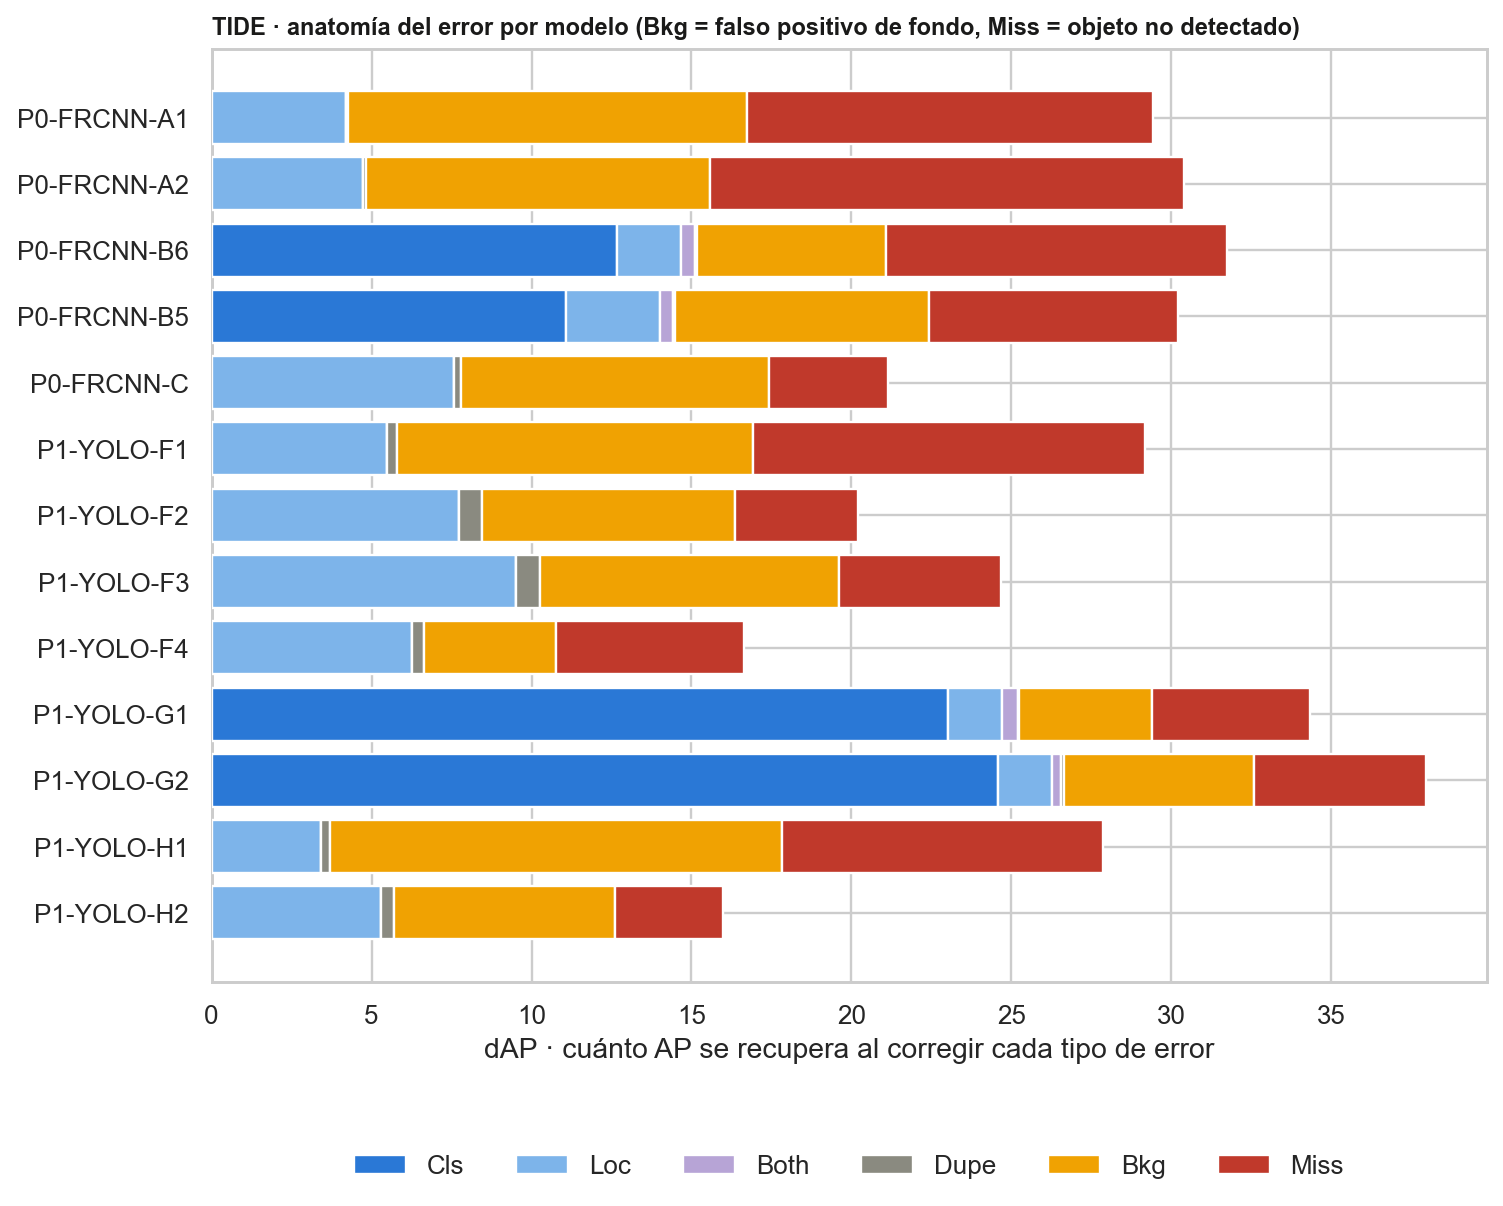
\includegraphics[width=\linewidth]{tide_descomposicion.png}
\caption{Descomposición de errores TIDE por modelo (dAP recuperado al corregir
cada tipo de error). Cls domina en los multiclase; Bkg+Miss en los de una
clase.}
\label{fig:tide}
\end{figure}

\subsection{Resultados cualitativos fuera de distribución}
La Figura~\ref{fig:demo} muestra la demo por lotes (notebook 07) sobre una
sesión de diez imágenes descargadas de internet, ajenas a los tres datasets.
Con umbrales conservadores (0.25 para YOLO, 0.5 para Faster R-CNN), los
patrones del protocolo cuantitativo reaparecen fuera de distribución: Faster
R-CNN propone más candidatos que YOLOv11n en las diez imágenes (211 contra 87
detecciones en total; 45 contra 15 en la escena más densa), el FCN estima entre
3 y 16\,\% de píxeles de basura por escena, y el clasificador VGG confirma cada
recorte con P(litter)$\ge$0.99, con Grad-CAM atendiendo al objeto y no a su
contexto. Estas imágenes son evidencia ilustrativa, no métrica: no poseen
anotaciones.

\begin{figure*}[t]
\centering
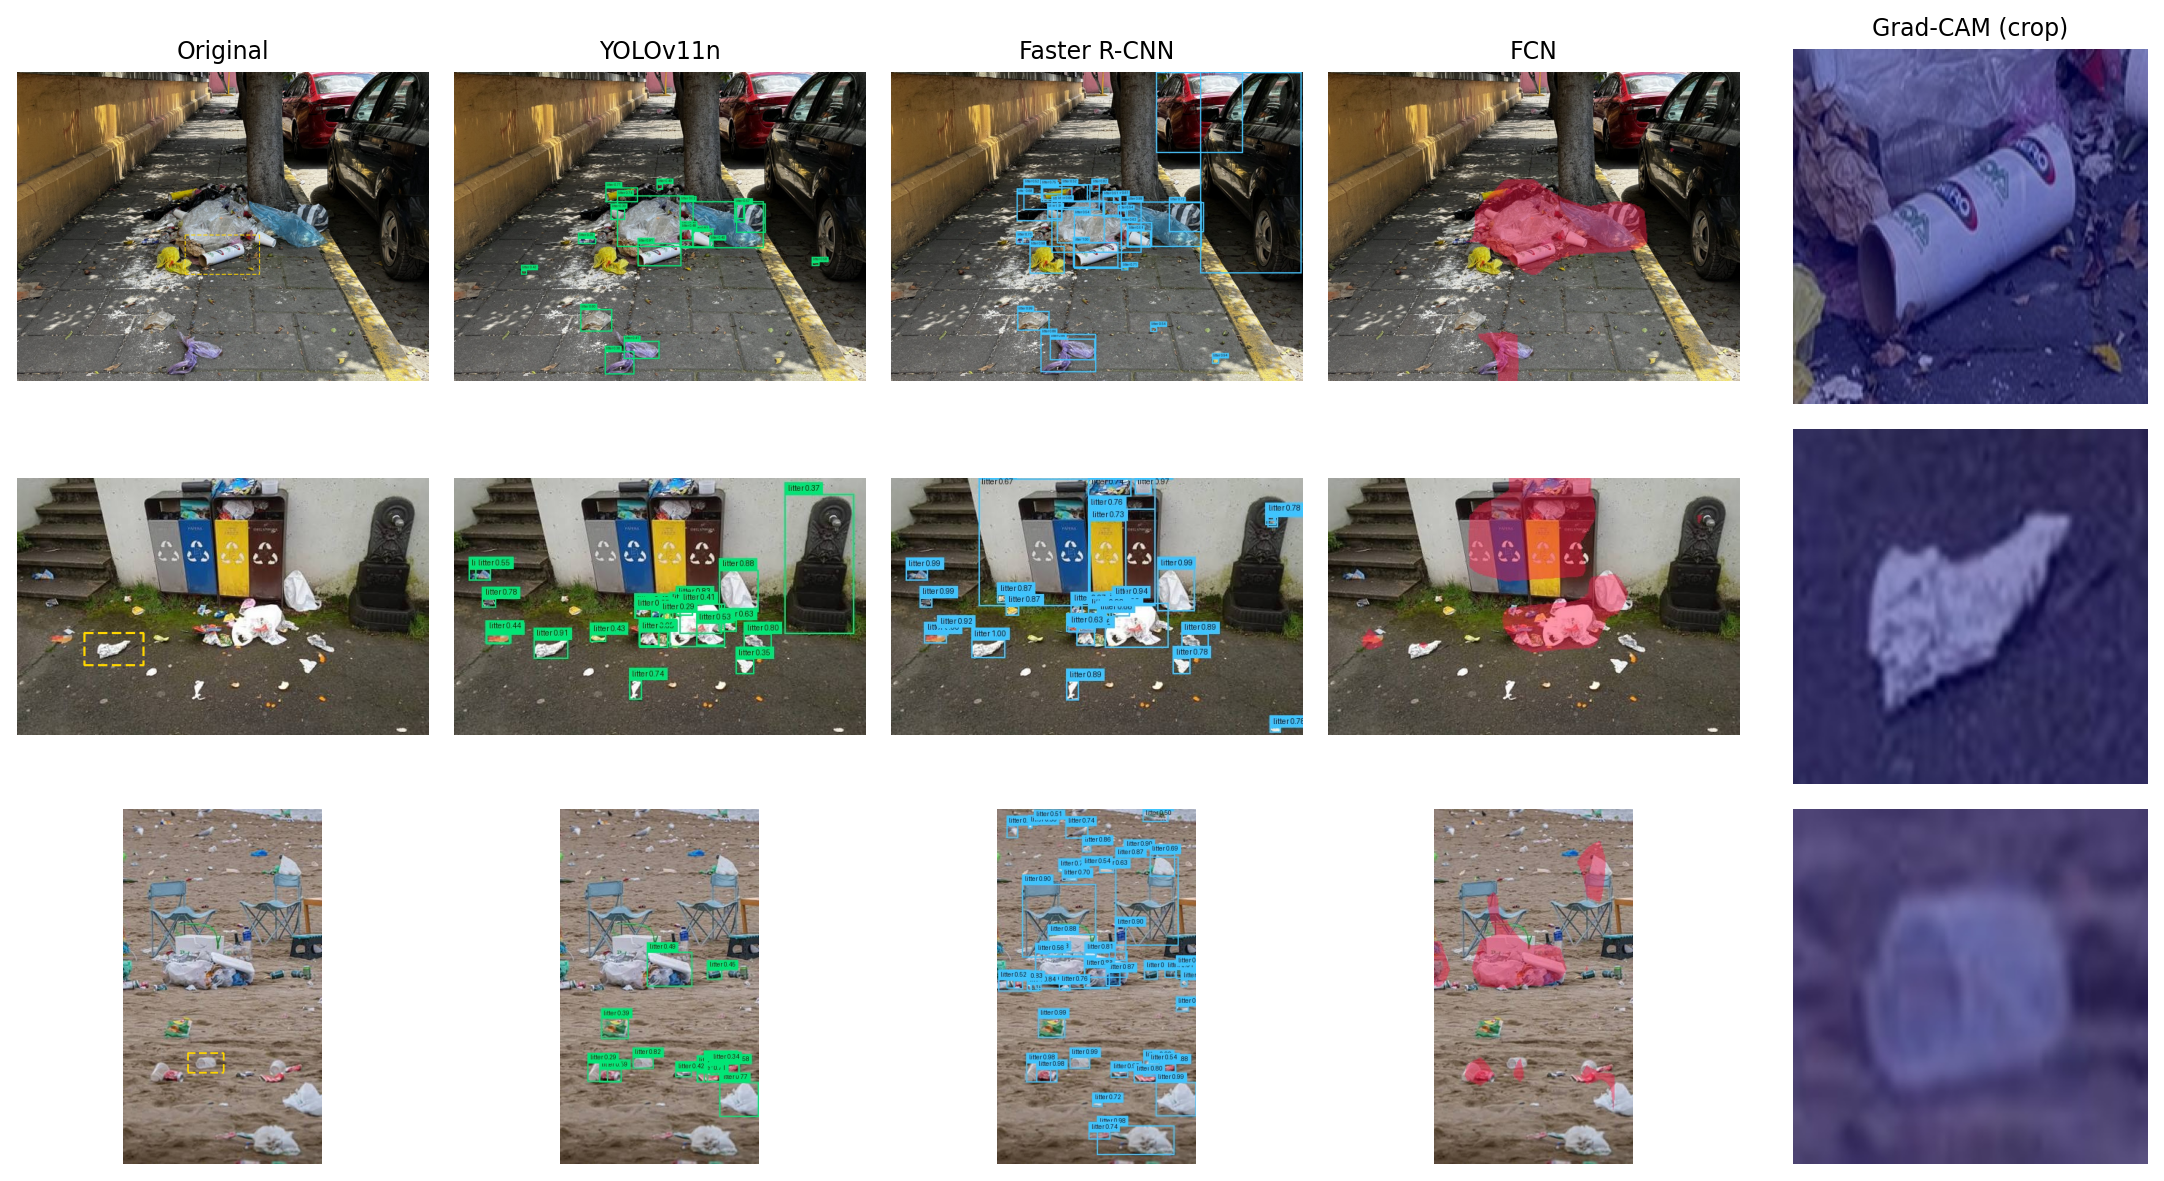
\includegraphics[width=\textwidth]{demo_cualitativa.png}
\caption{Demo cualitativa en imágenes web fuera de distribución (tres de las
diez de la sesión): original con el origen del recorte del Grad-CAM marcado en
punteado, detecciones YOLOv11n y Faster R-CNN, máscara FCN y explicación
Grad-CAM del clasificador de recortes. Imágenes descargadas aleatoriamente de
internet, sin metadata de autoría embebida, usadas únicamente con fines
ilustrativos; serán reemplazadas por capturas propias (Lima) en una revisión
futura.}
\label{fig:demo}
\end{figure*}

% =============================================================
\section{Discusión y limitaciones}
Tres hallazgos organizan la evidencia. \textbf{Los detectores de basura no
viajan.} La caída de 82\,\% entre dominios, con dashcam aislada y
mano$\leftrightarrow$dron parcialmente compatibles, se explica primero por la
escala del objeto: los dominios cuyos tamaños caen dentro del rango de anclas
del preentrenamiento intercambian algo de conocimiento; el régimen de 22\,px de
dashcam no intercambia nada. Para despliegues municipales con sensores mixtos,
el ajuste fino por dominio ---o al menos la adaptación de resolución--- sigue
siendo obligatorio; un modelo universal de basura aún no es realista.
\textbf{La higiene de los splits cambia conclusiones.} El protocolo oficial de
RoLID premia la memorización de escena (+21\,\% de AP$_{50}$); los resultados
publicados sobre él son optimistas en aproximadamente ese margen, y la
corrección (split por video, consciente de grupos) no cuesta nada. Sostenemos
que los datasets con estructura de video o ráfaga deberían publicar
identificadores de grupo. \textbf{Las palancas baratas funcionan.} La entrada de
1024\,px recompra +8.3 de AP$_{50}$ en dashcam; un detector de 2.6\,M de
parámetros rinde a pocos puntos de uno de 41.3\,M en detección de una clase; y
TIDE ubica el cuello de botella multiclase en la clasificación del material y no
en la localización ---lo que sugiere un diseño desacoplado (detector agnóstico a
la clase más clasificador de recortes, donde nuestro sustrato VGG alcanza
97.8\,\% de exactitud) por encima de cabezas de detección cada vez más finas.
Limitaciones que ya podemos enunciar: el mAP absoluto de este problema es
estructuralmente bajo~\cite{trashdet}; nuestro presupuesto de cómputo excluyó
detectores transformer (clase CO-DETR), que lideran el benchmark in-domain de
RoLID; StreetView-Waste no pudo incluirse (enlaces no disponibles); nuestra
propia captura fuera de distribución (Lima) queda como trabajo futuro, igual que
la agregación temporal sobre video de dashcam ---natural dada la estructura de
video que nuestra auditoría expuso.

% =============================================================
\section{Conclusión}
Auditamos tres datasets públicos de basura, publicamos splits corregidos
conscientes de grupos y medimos ---bajo un solo contrato de evaluación--- qué
tan lejos viajan los detectores de basura entre imágenes de mano, dashcam y
dron. Las respuestas son concretas: una caída de 82\,\% de mAP$_{50}$ fuera de
dominio con dashcam totalmente aislada; una inflación de +21\,\% de AP$_{50}$
escondida en los splits oficiales de RoLID-11K; hasta +8.3 de AP$_{50}$
recuperable solo con resolución de entrada; y un detector moderno 16$\times$ más
pequeño a pocos puntos de Faster R-CNN en basura de una clase. La descomposición
del error muestra que las batallas restantes son la discriminación del fondo y
la clasificación del material, no la localización. El pipeline completo ---de la
ingesta con checksums a las tablas generadas---, los pesos y una demo en vivo
son públicos; los detectores transformer, la agregación temporal sobre video de
dashcam y nuestra captura fuera de distribución planificada en Lima son los
siguientes pasos naturales.

\section*{Reproducibilidad}
Se publican el código, las notebooks (de la ingesta a la evaluación), los splits
auditados, los pesos entrenados y un video demo seccionado; se documentan tres
rutas de reproducción (demo con pesos preentrenados, regeneración de métricas
desde los artefactos publicados en $\sim$10 minutos, y reentrenamiento completo
desde los datos públicos). Los datasets se descargan de sus fuentes oficiales
con verificación de checksums.

\bibliographystyle{IEEEtran}
\bibliography{refs}

\end{document}
